%%%%%%%%%%%%%%%%%%%%%%%%%%%%%%%%%%%%%%%%%%%%%%%%%%%%%%%%%%%%%%%%%%%%%%%%%%%%%%%%%
%
% Purpose:  Verification part of V&V for the RadiationPressure model
%
%
%%%%%%%%%%%%%%%%%%%%%%%%%%%%%%%%%%%%%%%%%%%%%%%%%%%%%%%%%%%%%%%%%%%%%%%%%%%%%%%%

% \section{Verification}

%%% code imported from old template structure
%\inspection{<Name of Inspection>}\label{inspect:<label>}
% <description> to satisfy
% requirement \ref{reqt:<label>}.
\subsection{Top-level Requirement}

\inspection{Top-level Inspection}\label{inspect:top_level}
This document, the code, and associated files, have been inspected, and together
satisfy requirement ~\ref{reqt:top_level}.

\subsection{Inspection of Modeling Requirements}

\inspection{State Encapsulation}\label{inspect:stateencapsulation}
The model includes the capability to represent the relative state of the
vehicle, as demonstrated in section \vref{sec:verifflux}, thereby satisfying requirement \ref{reqt:stateencapsulation}

\inspection{Albedo Pressure}\label{inspect:albedopressure}
The foundation for the albedo pressure capability is provided in
\textit{RadiationSource::calculate\_flux}, utilizing the concept of third body
interactions, handled by class \textit{RadiationThirdBody}.  The method
\textit{RadiationThirdBody::calculate\_reflection\_flux} is not fully developed, but the output of this method can then be used in the appropriate \textit{incident\_radiation} method, which will increment, rather than overwrite, the calculated forces to ensure that multiple sources can be accumulated.  This satisfies requirement \ref{reqt:albedopressure}

\inspection{Force and Torque}\label{inspect:forceandtorque}
The data structures are populated by current force and torque values, as
required.  The legitimacy of those values is demonstrated in sections
\textref{Verification of Forces}{sec:verifforces} and \textref{Verification of
Flux}{sec:verifflux}.  This satisfies requirement \ref{reqt:forceandtorque}

\subsection{Verification of Surface Representations}

\test{Verification of two surface models} \label{test:surfacerepresentation}
\begin{description}
\item{Purpose:}\newline
To demonstrate that the \RadiationPressureDesc\ can interface with the Surface Model, and also operate separately from the Surface Model, using its own default surface representation.
\item{Requirements:}\newline
Satisfactory conclusion of this test satisfies requirement \ref{reqt:surfacerepresentation}
\item{Procedure:}\newline
A simulation was developed containing two independent radiation pressure models, one using the Surface Model, and the other one using the default surface model.  Both models were associated with the same vehicle, so the states were identical.  The vehicle was not propagated.
\item{Predictions:}\newline
Both surfaces should be initialized and a force calculated for each.  Since both surfaces have the same cross-sectional area, the forces should be comparable.
\item{Results:}\newline
Results are as expected.
\end{description}



\subsection{Verification of Force Calculations}\label{sec:verifforces}
The intent of this section is to show that the forces due to absorption, and
    specular and diffuse reflection are calculated correctly.
\test{Verification that the forces due to absorption, and
      specular and diffuse reflection are calculated correctly.}
  \label{test:Fasd}
  \begin{description}
  \item{Purpose:}\newline
    To test whether the calculations of the forces due to radiation absorption,
    and due to reflection through both specular and diffuse processes, are
    calculated appropriately.  While this particular test is applied to a surface comprising flat plates, other tests (\vref{test:surfacerepresentation}, and those in section \vref{sec:platemodelvalid}) demonstrate the similarity between the flat plate and the default surface representations.
  \item{Requirements:}\newline
    Satisfactory conclusion of this test, along with the tests~\ref{test:temperature_integration1} and ~\ref{test:temperature_integration2} satisfies requirement~\ref{reqt:functional_interaction}
  \item{Procedure:}\newline
    The simulation used in this test is available at \textit{SIM\_2\_SHADOW\_CALC/RUN\_ten\_plates}.
    A vehicle was built comprising 10 plates oriented at a range of angles with
    respect to the incident radiation, all illuminated, all of the time.  The
    forces were calculated for each plate with 50\% of the incident light being
    absorbed, and 25\% reflected through each of the diffuse and specular
    processes.
  \item{Predictions:}\newline
    \begin{enumerate}
    \item{Variation with time.}\ \newline
      The plates were held fixed with respect to the constant incident
      radiation vector; there should be no variation with time.
    \item{Component of force parallel to the flux vector.}
      \begin{itemize}
      \item{Calculation of force due to absorption.}\ \newline
        The only variable on which the force could depend is the angle,
				$\theta$, between
        the incident radiation and the plate normal.  This angle affects the
        projected area of the plate, and consequently should affect the force as
        the cosine of the angle.

        \begin{equation}
          F=F_{0} \cos \theta
        \end{equation}
        where $F_{0}$ is the force when $\theta = 0$.

      \item{Calculation of force due to specular reflection.}\ \newline
        There are two components contributing to the force {--} the incident and
        reflected light.  The incident magnitude will vary, as with the
        absorption, with the cosine of the angle.  The reflected magnitude
        will vary with the projected area ($\cos \theta$),
        and with the cosine of the double
        angle to account for the angle of reflection.  In this simulation,
        there is half as much light reflected specularly as absorbed, so the
        force looks like

\begin{equation*}
        F=\frac{F_{0}}{2}\cos \theta + \frac{F_{0}}{2}\cos \theta \cos 2\theta
\end{equation*}

        which simplifies to
        \begin{equation}
          F=F_{0} \cos ^{3}\theta
        \end{equation}

			  Here, $F_{0}$ maintains the same value defined for absorption.

			\item{Calculation of force due to diffuse reflection.}\ \newline
        Similarly to the specular reflection, there will be 2 components, but
        the angle of ``reflection'' will be along the normal, with
        value modified by the Lambert value of 2/3.
        \begin{equation}
          F=\frac{F_{0}}{2}\cos \theta \left(1+\frac{2}{3}\cos \theta \right)
        \end{equation}
      \end{itemize}

    \item{Component of force perpendicular to flux vector}
      \begin{itemize}
        \item{Calculation of force due to absorption.}\ \newline
           The component of force due to absorption perpendicular to the flux
           vector should be zero.
        \item{Calculation of force due to specular reflection.}\ \newline
           The magnitude depends on the projected area again, but only has
           contribution from the reflected component (the incident
           component is parallel to the flux vector, by definition).

         \begin{equation}
           F=\frac{F_{0}}{2}\cos \theta \sin 2\theta
         \end{equation}

        \item{Calculation of force due to diffuse reflection.}\ \newline
          Similarly, the magnitude depends on the projected area
          and the contribution from the reflected component only.

          \begin{equation}
            F=\frac{F_{0}}{2}\cos \theta \left(\frac{2}{3}\sin \theta
              \right)=\frac{F_{0}}{6}\sin 2\theta
          \end{equation}
      \end{itemize}
    \end{enumerate}
  \item{Results:}\newline
    \begin{enumerate}
      \item{} As expected, there was no variation with time.
      \item{}
        Figure~\ref{fig:ivv_F_asd_values_par} shows
        the data for the parallel component of the force for each of the three
        processes.  All 3 variables match their analytical predictions.
      \item{}
        Figure~\ref{fig:ivv_F_asd_values_perp} shows
        the data for the perpendicular component of the force for each of the
        three processes.  All 3 variables match their analytical predictions.
    \end{enumerate}
    \begin{figure}[!ht]
        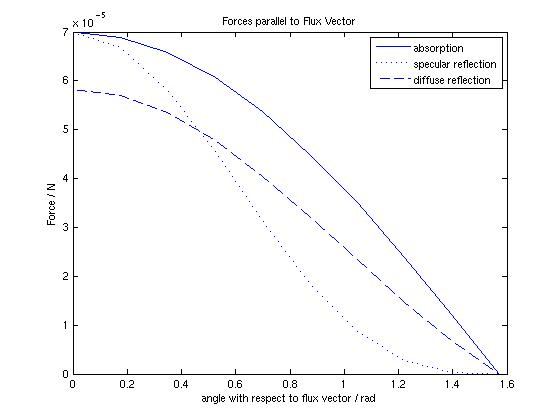
\includegraphics[width=180mm]{figs/Fsda/forces_parallel.jpg}
        \caption{The components of the absorption, specular, and diffuse forces
        parallel to the flux vector as a function of the angle between the flux
        vector and the surface normal}
        \label{fig:ivv_F_asd_values_par}
    \end{figure}

    \begin{figure}[!ht]
        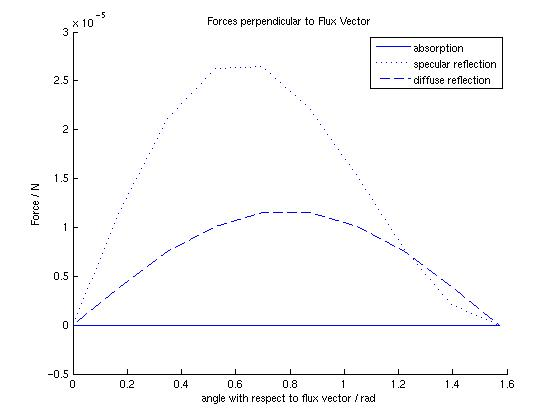
\includegraphics[width=180mm]{figs/Fsda/forces_perpendicular.jpg}
        \caption{The components of the absorption, specular, and diffuse forces
        perpendicular to the flux vector as a function of the angle between the
        flux vector and the surface normal}
        \label{fig:ivv_F_asd_values_perp}
    \end{figure}
  \end{description}

  \clearpage

\subsection{Verification of the Temperature Integration and Thermal
Emission Procedures}\label{test:temperature}

  This section is divided into two parts, one comparing the case of
  the vehicle without illumination --- for which an analytic solution
  exists --- and the second comparing the response of surfaces with different
  characteristics in the presence of illumination.

  \subsubsection{Verification of Thermal Processes without Illumination}
  \test{Thermal Processes - no illumination}
  \label{test:temperature_integration1}
  \begin{description}
  \item{Purpose:}\ \newline
    This test is to ensure that the Runge-Kutte plate-temperature integration
    process is functioning normally in the case of a vehicle cooling in the
    absence of incident radiation.
  \item{Requirements:}\ \newline
    Satisfactory conclusion of this test, along with test~\ref{test:temperature_integration2} satisfies requirements~\ref{reqt:functional_temperature} and~\ref{reqt:temperaturestructure}.

    Satisfactory conclusion of this test, along with the tests~\ref{test:temperature_integration2} and ~\ref{test:Fasd} satisfies requirement~\ref{reqt:functional_interaction}.
  \item{Procedure:}\ \newline
    The simulations used in this test are available at \textit{SIM\_2\_SHADOW\_CALC/RUN\_shadow\_cooling} (for the regular Surface Model surface) and at \textit{SIM\_2A\_SHADOW\_CALC/RUN\_shadow\_cooling} (for the default surface).
    For the Surface Model, a number of plates were monitored in a flux-free environment to observe
    their temperature variation with time, and the effect of that temperature
    variation on the variation of the emissive force with time.  Each plate had
    slightly different characteristics, allowing for the dependency on
    emissivity, plate area, and heat capacity to be investigated.  For the second simulation, a default surface was placed in the same environment.  In the
    absence of incident flux, an analytic solution exists for the temperature
    and the force, and this can be compared to the numerical solution.
  \item{Results:}
    \begin{enumerate}
    \item{Variation with time of force}\newline
      As expected, the absorption, diffuse, and specular forces were all zero
      for the duration of this simulation.
      The emission forces matched well with analytic predictions (see Figure~\ref{fig:forceanalytic}, and had the
      correct orientation.
    \item{Variation with time of temperature}\newline
      Simulation data matched very well to analytic solution.  On any scale
      longer than 3 timesteps, the graphs of analytical values and simulation
      values were indistinguishable, with a difference less than 0.05\%, and
      very much smaller than the observed changes in temperature.  See Figure~\ref{fig:temperatureanalytic}.
    \item{Variation with emissivity of the temporal evolution of temperature}\newline
      As the emissivity increases, the rate of change of temperature also
      increases, as expected.  For $\epsilon$=0, no temperature
      change was observed.
    \item{Variation with starting temperature of the temporal evolution of temperature}\newline
      With a lower starting temperature, a plate maintains a lower temperature
      throughout the simulation, but the temperature decreases more slowly.
      Temperature$\sim$time plots have identical shapes; shifting the curves along
      the x-axis to match temperature at some time results in matching
      temperatures for all (valid) time.
    \item{Variation with plate area of the temporal evolution of temperature}\newline
      A plate with a smaller surface area, but identical heat capacity shows a
      more gradual temperature drop.  There is no observable difference between
      plates for which the heat capacity is decreased proportionally with the
      area (e.g. smaller plate of the same material).
    \item{Variation with heat capacity of the temporal evolution of temperature}\newline
      A plate with a smaller heat capacity, but identical area shows a
      more rapid temperature drop.  There is no observable difference between
      plates for which the area is decreased proportionally with the heat
      capacity (e.g. smaller plate of the same material).
    \end{enumerate}

    \begin{figure}
         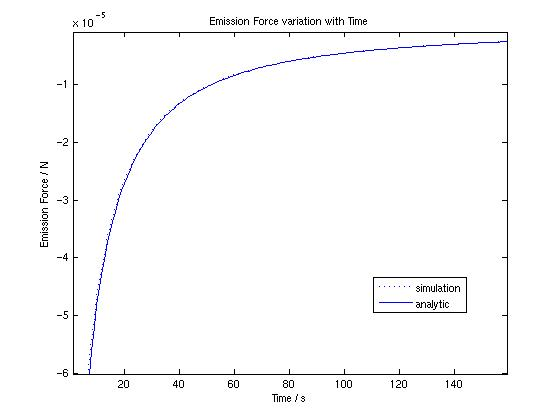
\includegraphics[width=180mm]{figs/Fe_int/force_analytic.jpg}
         \caption{Variation with time of force, showing the simulation data
         and analytic solution overlaying.}
         \label{fig:forceanalytic}
    \end{figure}
    \begin{figure}
         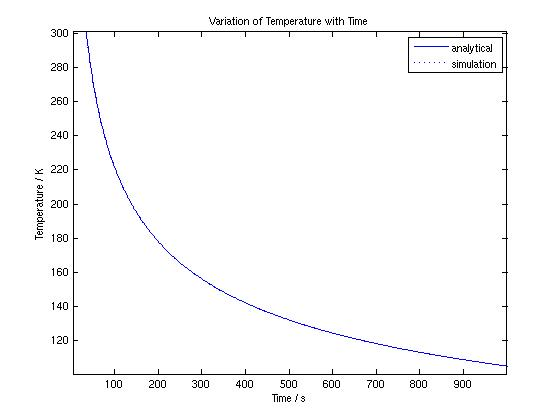
\includegraphics[width=180mm]{figs/Fe_int/temperature_analytic.jpg}
         \caption{Variation with time of temperature, showing the simulation data
         and analytic solution overlaying.}
         \label{fig:temperatureanalytic}
    \end{figure}

  \end{description}
  \clearpage

  \subsubsection{Verification of Thermal Processes with Illumination}
  \test{Thermal Processes - with illumination}
  \label{test:temperature_integration2}
  \begin{description}
  \item{Purpose:}\ \newline
    To verify that the temperature integration and thermal emission processes
    are functioning as expected when the vehicle is illuminated.
  \item{Requirements:}\ \newline
    Satisfactory conclusion of this test, along with test~\ref{test:temperature_integration1} satisfies requirements~\ref{reqt:functional_temperature} and~\ref{reqt:temperaturestructure}.

    Satisfactory conclusion of this test, along with the tests~\ref{test:temperature_integration1} and ~\ref{test:Fasd} satisfies requirement~\ref{reqt:functional_interaction}.
  \item{Procedure:}\ \newline
  The simulation used in this test is available at \textit{SIM\_2\_SHADOW\_CALC/RUN\_ten\_plates}.
    Ten identical plates were oriented at different angles to the flux
    vector, with the angle between the normal and the flux vector varying
    from 0 to 90 degrees.  All plates were started with a preliminary
    temperature of 270 K, and the simulation was allowed to run until all but
    one plate had approached their equilibrium temperature.  The force from each plate
    was monitored throughout the simulation.
  \item{Results:}\ \newline
    The equilibrium temperature is calculated from the energy balance equation
    \begin{equation}
      \phi (A\cos \theta )(1-\alpha )=\epsilon \sigma A{T_{\mathit{eq}}}^{4}
    \end{equation}

    where
    \begin{itemize}
      \item{}
        $\phi$ is the radiative flux,
      \item{}
        $\theta$ is the angle between the surface normal and the incident
        radiation vector,
      \item{}
        $\alpha$ is the albedo of the surface,
      \item{}
        $\epsilon$ is the emissivity of the surface,
      \item{}
        $\sigma$ is the Stefan-Boltzmann constant,
      \item{}
        A is the plate area, and
      \item{}
        $T_{\mathit{eq}}$ is the equilibrium temperature.
    \end{itemize}

    Using values of $\alpha =0.5$,  $\epsilon =0.5$, $\phi =
    1400~W~ m^{-2}$, and with $\theta$ varying from 0 to 90 degrees in 10 degree
    intervals, the equilibrium temperatures of the 10 plates are:

    396 K, 395 K, 390 K, 382 K, 371 K, 355 K, 333 K, 303 K, 256 K, and 0 K.

    Figure~\ref{fig:ivv_F_emission_Tint} shows the variation with time of the
    temperature of the 10 plates; the 9 plates that had closely approached equilibrium temperatures had
    final temperatures all within
    1\% of their analytical equilibrium temperature.

      \begin{figure}[!ht]
        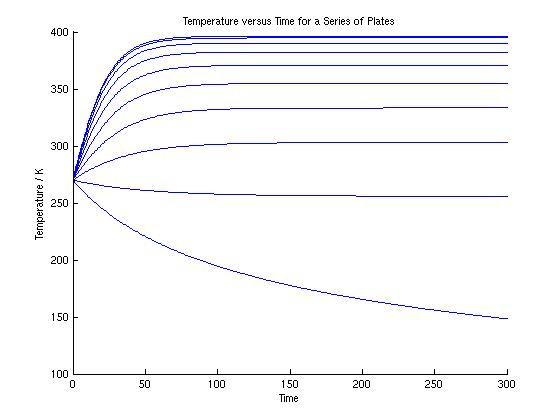
\includegraphics[width=180mm]{figs/Fe_int/temperature-time.jpg}
        \caption{The variation of temperature with time over the 10 plates in
        the simulation.}
        \label{fig:ivv_F_emission_Tint}
      \end{figure}

    The final plate, with an equilibrium temperature of 0 K has a temperature
    variation that is decreasing at a rate consistent with expectations.

    The force due to emission should be directed opposite to the surface
    normal, and have magnitude equal to the ratio of power emission to speed of
    light, producing equilibrium values of 47, 46, 44, 40, 36, 30, 23, 16, 8,
    and 0  ${\mu}$N.

    Figure~\ref{fig:ivv_F_emission_10plate} shows the variation with
    time of the force due to emission, confirming the analytic
    values.
    \begin{figure}[!ht]
        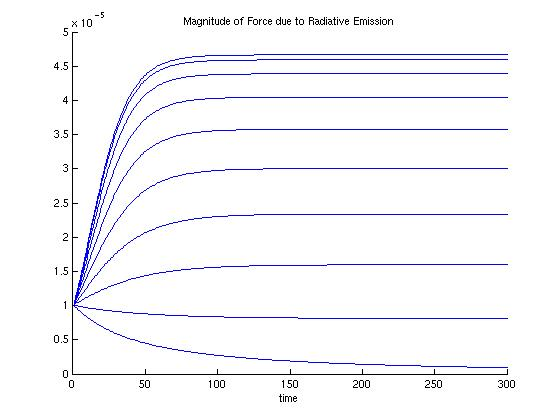
\includegraphics[width=180mm]{figs/Fe_int/force_emission10plate.jpg}
        \caption{The variation with time of force, over the 10 plates in
        the simulation.}
        \label{fig:ivv_F_emission_10plate}
      \end{figure}
  \clearpage
  \end{description}
\clearpage

\subsection{Verification of the Flux Calculations}\label{sec:verifflux}

This section is divided into two parts:  the first considers a
vehicle in Earth's shadow at several locations along the extension
of the Sun-Earth
vector, the second considers a vehicle moving perpendicular to the
Sun-Earth vector, passing through Earth's shadow.

  \subsubsection{Eclipse calculations along the extension of the Sun-Earth vector}
    \test{Verification of the eclipse calculation for an object
      moving along the Sun-planet axis through the region of annular eclipse}
    \label{test:eclipse_annular}
    \begin{description}
      \item{Purpose:}\ \newline
        The purpose of this simulation is to confirm that the code
        correctly identifies and calculates the extent of shadowing by an
        intervening body.
      \item{Requirements:}\ \newline
        The results of this test, together with the results
        from~\ref{test:eclipse_transverse}, together satisfy
        requirement~\ref{reqt:functional_eclipse}.
      \item{Procedure:}\ \newline

The simulation used in this test is available at \textit{SIM\_2\_SHADOW\_CALC/RUN\_annular\_eclipse}.
        The vehicle was placed at various locations along the dotted line shown
        in figure~\ref{fig:ivv_annular_eclipse_layout}.

        \begin{figure}[!ht]
          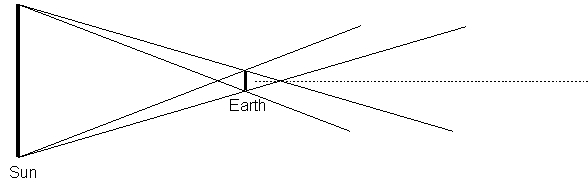
\includegraphics[width=180mm]{figs/eclipse/annular_eclipse_layout.jpg}
          \caption{The location of the vehicle, with respect to Earth and Sun,
                 during the simulation.}
          \label{fig:ivv_annular_eclipse_layout}
        \end{figure}
        Two runs were made:
        \begin{enumerate}
          \item{} the first used the cylindrical shadow model,
          \item{} the second used the conical shadow model.
        \end{enumerate}
          The value of the flux vector was evaluated at several
          locations for each run.
      \item{Results:}\ \newline
        Both runs produced results entirely in line with expectations.
        \begin{enumerate}
          \item{}
            For the first run (cylindrical shadow), there was no illumination at any location on
            the line.
          \item{}
            For the second run (conical shadow), there was no illumination while the vehicle
            was inside the cone representing totality.
            At larger distances, the magnitude of the flux increased as a
            greater percentage of the solar disk became visible; at very
            large distances from Earth ($>10^{10}$  m), the flux magnitude
            decreased with distance due to the inverse-square nature of
            the flux magnitude and the fact that the fraction of the solar
            disk that is exposed changes only very slowly at these distances.
            The data matched the theoretical predictions very closely.
            \begin{figure}[!ht]
       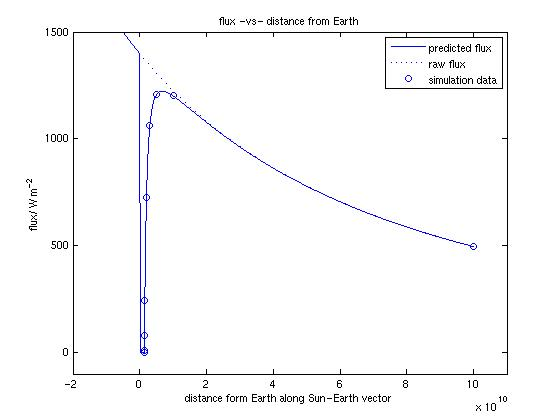
\includegraphics[width=180mm]{figs/eclipse/flux-radial_distance.jpg}
              \caption{The flux of the vehicle as a function of distance
                from Earth on the Sun-Earth vector.  The raw flux represents
                the solar flux without shadowing.  The predicted flux
                represents the analytic function
                for flux with Earth shadowing included.  Data points from the
                simulation are shown as circles.}
              \label{fig:ivv_flux_radial_distance}
            \end{figure}
        \end{enumerate}
     \end{description}
\clearpage

  \subsubsection{Eclipse calculations perpendicular to the extension of the
     Sun-Earth vector}
  \test{Verification of the eclipse calculation for an object
    moving across the region of total eclipse}
  \label{test:eclipse_transverse}
  \begin{description}
    \item{Purpose:}\newline
      The purpose of this simulation is to confirm that the code
      correctly identifies and calculates the extent of shadowing by an
      intervening body.
    \item{Requirements:}\newline
        The results of this test satisfy
        requirement~\ref{reqt:functional_flux}, and together with the results
        from~\ref{test:eclipse_annular}, satisfy
        requirement~\ref{reqt:functional_eclipse}.
    \item{Procedure:}\newline

The simulation used in this test is available at \textit{SIM\_2\_SHADOW\_CALC/RUN\_transverse\_shadow}.
      Two different techniques were used to investigate the
      response to the position within the shadow of the planet.
      \begin{enumerate}
        \item{}
        A series of runs was made with the vehicle traversing the shadow,
        perpendicular to the Sun{}-Earth vector at a selection of values of
        $r_{\mathit{par}}$, the component of the Earth-vehicle vector parallel to
        the Sun-Earth vector, as shown in
        Figure~\ref{fig:ivv_transverse_eclipse_layout}.
        The simulation included in the \JEODid\ release corresponds to line number 4 in this description.  With an Earth-vehicle distance of $1.35 \times 10^9 m$, this corresponds to the apex of the cone representing totality.  Line number 1 in this description is actually located at a distance of $1.35 \times 10^4 m$ from the center of Earth.  This value is well within the planet; values closer to the planet center had complicating issues associated with Earth moving on its orbit during the simulation in such a way that the position of the vehicle was closer to Sun than was Earth.
        \begin{figure}[!ht]
          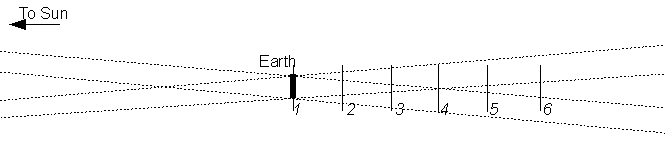
\includegraphics[width=180mm]{figs/eclipse/drawings1_te.jpg}
          \caption{The 6 paths of the vehicle across Earth's shadow}
          \label{fig:ivv_transverse_eclipse_layout}
        \end{figure}

        \item{}
        Another run was made in which the inertial position of the
        vehicle was held fixed with respect to Earth, and the ephemeris allowed to evolve.
        Starting with the vehicle in the conical shadow, it gradually moved
        into full sunlight as the earth moved around its orbit, as shown in
        Figure~\ref{fig:ivv_transverse_eclipse_layout2}.


        \begin{figure}[!ht]
          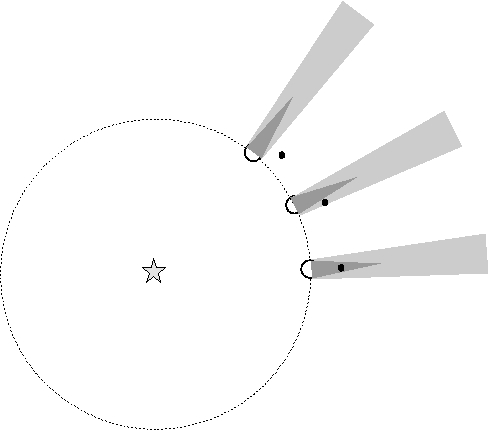
\includegraphics[width=80mm]{figs/eclipse/drawings2_te.jpg}
          \caption{The position of the vehicle with respect to Sun as it transits
            Earth's shadow.}
          \label{fig:ivv_transverse_eclipse_layout2}
        \end{figure}
      \end{enumerate}

    \item{Results:}\newline
    \begin{enumerate}

      \item{}
      In the first run (vehicle passes through Earth shadow), the Sun-vehicle vector changes in both direction and
      magnitude, thus
      affecting the flux unit vector (flux\_hat), the magnitude of the flux
      vector, and each individual component of the flux vector; these changes
      were consistent with theory.

    The six lines in Figure~\ref{fig:ivv_flux_transverse_eclipse}
    each represent the magnitude of the force
    experienced by a vehicle as it traverses Earth's shadow.  Each line
    represents a different value of $r_{\mathit{par}}$ and is
    shown as a function of $r_{\mathit{perp}}$, the component of the
    Earth-vehicle vector that is perpendicular to the Sun-Earth vector.

    For passes that were sufficiently close to Earth that the vehicle passed through the region of totality (i.e. passes 1-3, with pass 4 satisfying this requirement only momentarily), we see the effects of both umbral and penumbral shadowing.  The penumbral (partial shadowing)
    region is indicated by a sloping line; the umbral (total shadowing) region
    is indicated by a flat line and zero force.

    The first line (corresponding to a vehicle passing close to the center of Earth) shows no penumbral region, and an umbral region equal in
    size to Earth.  Getting farther from Sun, the extent of the penumbral
		region grows, and that of
    the umbral region shrinks until it disappears by the fourth line, which is the limit of total eclipse.  Farther yet from Earth, passes 5 and 6 represent annular eclipses, with the angular size of Earth now
		smaller than that of the sun.  Annular eclipses do not have umbral regions; instead the flux should fall until the intervening body is completely within the solar disk, then stay constant as the intervening body traverses the solar disk, then rise again as it leaves the disk.  Pass 6 in particular shows the annular eclipse lasting for some distance at
    constant illumination.  Also, evident in the wings of the first three lines,
    beyond the points of total illumination, is the gradual decrease in
    illumination due to increased distance from Sun.

    \begin{figure}[!ht]
      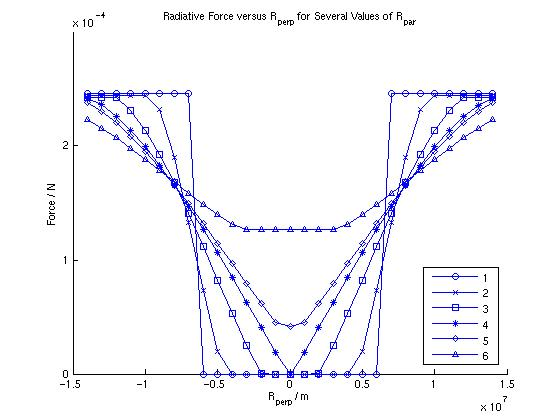
\includegraphics[width=180mm]{figs/eclipse/force_partial_eclipse.jpg}
      \caption{The magnitude of the radiative force as a function of
      $r_{\mathit{perp}}$ for different values of $r_{\mathit{par}}$}
      \label{fig:ivv_flux_transverse_eclipse}
    \end{figure}

    \item{}
      The second simulation (shadow moves with respect to a fixed-orientation of Earth and vehicle) demonstrated very similar results, with
      almost-negligible changes in the Sun-vehicle distance, and
      hence in the raw flux magnitude throughout the simulation.
    \end{enumerate}
  \end{description}
\clearpage


\subsubsection{Confirmation of eclipsing bodies}
\inspection{Vehicle can be shadowed by any intervening body.}\ \newline
\label{inspect:eclipsingbody}
The functionality to calculate the effect of an eclipsing body is demonstrated in tests~\vref{test:eclipse_annular} and \vref{test:eclipse_transverse}.  The flexibility to include shadowing of more than one body is found in \textit{RadiationSource::calculate\_flux}, although this is not complete;  where two intervening bodies overlap, the code will calculate the fractional part of the disk that is visible behind each (e.g. 90\% and 80\%) and multiply these together (72\%).  If the two bodies are blocking the same part of the disk, this is an invalid number.  For a fully correct implementation, the ``shadowing'' of third-bodies by third-bodies also needs to be considered.  Nevertheless, the requirement is for this functionality to be available as an extension, and in that sense, this inspection satisfies requirement~\ref{reqt:eclipsingbody}.
